\documentclass[titlepage]{article}
\usepackage{graphicx}
\usepackage[tbtags]{amsmath}

\begin{document}

\title{Experiment 2: Measurement of $g$}
\author{Tian Ye \\ \\ UID: 704931660 \\ \\ TA: Wen Li Wen \\ \\ Lab Partners: \\ \\ Matthew Barba, Dong Han,\\ \\ Chris Ong, Edward Xie \\ \\ Lab 8 Tuesday 6:00 PM}
\date{October 17th, 2017}

\maketitle

\section{Ball Drop}
\subsection{Introduction}
The premise of the ball drop half of Experiment 2 is to measure \textit{g}, the gravitational constant of Earth, by dropping a ball through a setup of two photogates and an impact sensor and measuring the elapsed time the ball takes traveling between the two photogates and the second photogate to the impact sensor on the bottom. A diagram of the setup is shown below:

\begin{figure}[!htbp]
    \centering
    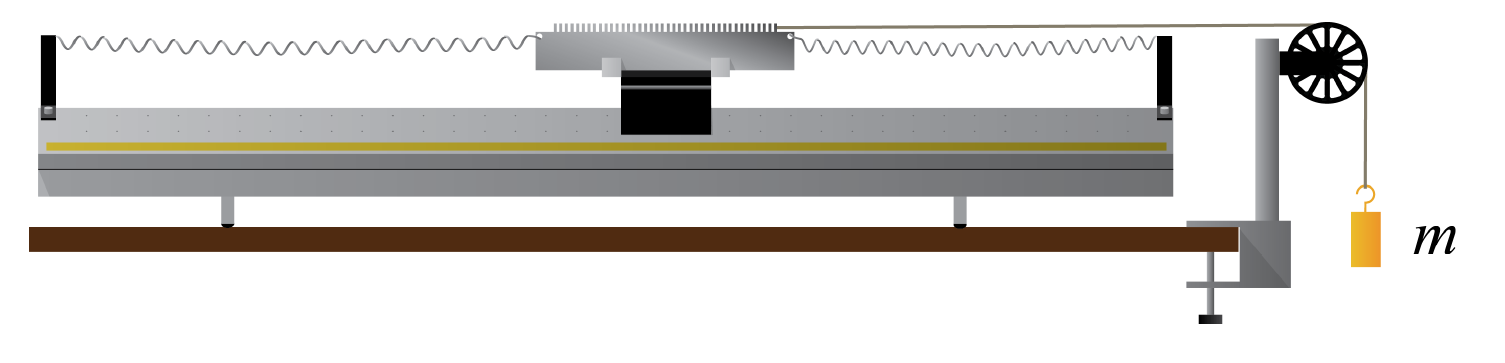
\includegraphics[width=3.0in]{Setup.png}
    \caption{Visual representation of the photogates and impact sensor system. Figure reproduced
(with permission) from Fig. 2.1 by Campbell, W. C. \textit{et al.\textsuperscript{1}}.}
\end{figure}

\subsection{Solving for \textit{g}}
Referencing the above diagram, we will define the distance between the two photogates as \textit{d} and the distance between the second photogate and the impact sensor as \textit{D}, and the time the ball takes to travel between the two sections as t\textsubscript{1} and t\textsubscript{2}, respectively. Using kinematics and assuming \textit{g} to be constant, we can define two seperate equations with two unknowns, v\textsubscript{0} and \textit{g}, and solve for \textit{g}. The two equations we define are as follows:

\begin{equation}
    \begin{aligned}
         d &= v_0 t_1 + \frac{1}{2}g t_1\textsuperscript{2} \\
        (d + D) &= v_0(t_1 + t_2) + \frac{1}{2}g(t_1 + t_2)
    \end{aligned}
\end{equation}

\pagebreak

Isolating $v_0$ for both equations, we can in turn set them equal to each other and solve for \textit{g}, presenting us with the following:

\begin{equation}
    \begin{split}
        \frac{d-\frac{1}{2}g t_1\textsuperscript{2}}{t_1} &= \frac{d + D-\frac{1}{2}g(t_1 + t_2)^2}{t_1 + t_2} \\
        g &= \frac{2}{t_1+t_2} \bigg ( \frac{D}{t_2} - \frac{d}{t_1} \bigg )
    \end{split}
\end{equation}

Inputting the collected data values into Equation 2 which was defined above, we find the following values for \textit{g}:

\begin{table}[!htbp]
\renewcommand{\arraystretch}{1.3}
\centering
\scalebox{0.7}
{
\begin{tabular}{c|c|c}
    \hline
    \hline
    D (Height in mm) & Calculated \textit{g} (m/s$^2$) & Average \textit{g} (m/s$^2$)\\
    \hline
    \hline

    243 $\pm$ 1 &  9.63, 9.63, 11.05, 11.05, 12.67, 9.32, 9.32, 9.32, 9.63, 9.63 &  10.12 \\
    \hline

    381 $\pm$ 1 & 9.42, 10.99, 10.15, 10.15, 10.99, 10.99, 10.14, 10.14, 10.14, 10.70 &  10.38 \\
    \hline

    448 $\pm$ 1 & 9.60, 9.60, 9.60, 9.60, 10.20, 10.20, 10.10, 9.60, 8.80, 10.10 &  9.73 \\
    \hline

    563 $\pm$ 1 &  9.98, 9.98, 9.98, 9.98, 9.37, 9.98, 9.98, 9.27, 8.16, 8.16 &  9.48 \\ 
    \hline

    653 $\pm$ 1 &  10.36, 10.36, 8.73, 10.36, 10.36, 9.72, 9.72, 9.72, 9.72, 9.39 &  9.85 \\
    \hline
\end{tabular}
}
\caption{Data for the ball drop portion of the experiment. Note that in all trials of the experiment, \textit{d} remained unchanged at a value of 85 $\pm$ 1 mm. The uncertainties in the measurements of \textit{d} and \textit{D} are due to systematic uncertainties.}
\end{table}

However, the data above is incomplete, as it lacks the uncertainties for the calculated values of \textit{g}.

\subsection{Solving for Uncertainty of \textit{g}}
Solving for uncertainty of \textit{g} is rather convoluted in this particular scenario as there is both statistical and systematic uncertainty.

\subsubsection{Statistical Uncertainty}
To solve for statistical uncertainty, we will use the formula ii.13 from the lab manual, being the following:

\begin{align}
     \delta g = \frac{\sigma\textsubscript{g}}{\sqrt{N}}
\end{align}

Where $\sigma_g$ is the sample standard deviation of \textit{g} and \textit{N} is the number of data points. 

\pagebreak

Using the values in Table 1, we then find the statistical uncertainty shown in the table below:

\begin{table}[!htbp]
\renewcommand{\arraystretch}{1.3}
\centering
\begin{tabular}{c|c}
    \hline
    \hline
    D (Height in mm) & Sample Statistical Uncertainty (m/s$^2$)\\
    \hline
    \hline

    243 $\pm$ 1    &  0.11 \\
    \hline

    381 $\pm$ 1    &  0.05 \\
    \hline

    448 $\pm$ 1   &  0.04\\
    \hline

    563 $\pm$ 1   &  0.07\\
    \hline

    653 $\pm$ 1  &  0.05\\
    \hline
\end{tabular}
\caption{\textit{d}, not included in the table, has a value of 85 $\pm$ 1 mm.}
\end{table}

\subsubsection{Systematic Uncertainty}
As there are uncertainties in both \textit{d} and \textit{D}, we will solve for \textit{g} again, this time maximizing and minimizing \textit{g} via using the upper and lower limits of \textit{d} and \textit{D}. The upper and lower limits of the distance values are found by taking the best measurements of the distance and adding or subtracting the uncertainty of the distance. Looking at Equation 2, it can be seen that \textit{g} is maximized when \textit{d} is minimized and \textit{D} is maximized. The reverse holds true as well: \textit{g} is minimized when \textit{d} is maximized and \textit{D} is minimized. Using then the formula

\begin{align}
    \delta g = \frac{g\textsubscript{max} - g\textsubscript{min}}{2}
\end{align}

we can solve for the systematic portion of the uncertainty, which is shown on the table below:

\begin{table}[!htbp]
\renewcommand{\arraystretch}{1.3}
\centering
\begin{tabular}{c|c}
    \hline
    \hline
    D (Height in mm) & Systematic Uncertainty (m/s$^2$)\\
    \hline
    \hline

    243 $\pm$ 1    &  0.26 \\
    \hline

    381 $\pm$ 1    &  0.17 \\
    \hline

    448 $\pm$ 1   &  0.14\\
    \hline

    563 $\pm$ 1   &  0.13\\
    \hline

    653 $\pm$ 1  &  0.11\\
    \hline
\end{tabular}
\caption{\textit{d}, not included in the table, has a value of 85 $\pm$ 1 mm. The systematic uncertainty was obtained by averaging all the uncertainties for the 10 data points for each particular height, \textit{D}.}
\end{table}

\subsubsection{Total Uncertainty}
From the statistical and systematic uncertainty values, we can begin to derive total uncertainty. The value for total uncertainty of \textit{g} is derived from the summation of the statistical and systematic uncertainties of \textit{g}. However, in the event that one of the uncertainties differs from the other by a factor of 10 or more, the smaller uncertainty may be ignored, as the smaller value would be discarded nonetheless when significant figures are taken into account. 

In this particular scenario the statistical uncertainty, which is for all data values less than the systematic uncertainty, does not differ from the systematic uncertainty by a factor greater than 10; therefore, the total uncertainty will be a summation of the two:

\begin{table}[!htbp]
\renewcommand{\arraystretch}{1.3}
\centering
\begin{tabular}{c|c}
    \hline
    \hline
    D (Height in mm) & Calculated \textit{g} with Uncertainty (m/s$^2$)\\
    \hline
    \hline

    243 $\pm$ 1    &  10.12 $\pm$ 0.37 \\
    \hline

    381 $\pm$ 1    &  10.38 $\pm$ 0.22 \\
    \hline

    448 $\pm$ 1   &   9.73 $\pm$ 0.18\\
    \hline

    563 $\pm$ 1   &  9.48 $\pm$ 0.20\\
    \hline

    653 $\pm$ 1  &  9.85 $\pm$ 0.16\\
    \hline
\end{tabular}
\caption{\textit{d}, not included in the table has a value of 85 $\pm$ 1 mm. The final values for \textit{g} are displayed above, with their corresponding uncertainties.}
\end{table}

\pagebreak

\subsection{Data Analysis}

From our knowledge of physics, we know that \textit{g} should not depend on \textit{D}, as the gravitational constant is a constant. Below is a plot of \textit{g} against \textit{D}

\begin{figure}[!htbp]
    \centering
    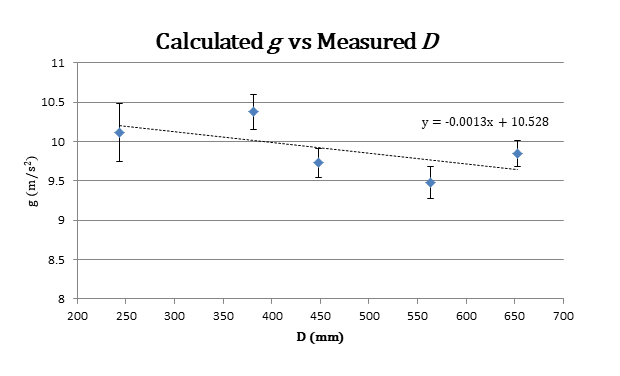
\includegraphics[width=5.0in]{Chart.png}
    \caption{Measured acceleration due to gravity plotted against D, with error bars representing the uncertainty associated with each value of \textit{g}. The uncertainty of the slope is .0009}
\end{figure}

When we view the graph, we see that although there appears to be no correlation between \textit{g} and \textit{D}, the value of $\delta$g seems to increase as \textit{D} approaches 0. Viewing the equation of the linear regression provided by Microsoft Excel, we see that the slope provided, -.0013, is not consistent with zero as the value of the uncertainty, .0009, does not overlap with zero with combined with the slope. Nonetheless, the slope is of such a small value that the trend can be attributed to various systematic errors discussed below.

In light of these observations, we can state that the limitations in the experiment are a result of limitations in the precision of measurement, as when we view uncertainty, we see that the systematic uncertainty is far greater than the statistical uncertainty. Furthermore, we can also safely state that the inconsistencies cannot be completely attributed to air resistance, as the force of air resistance is related to the velocity. This in turn suggests that for greater \textit{D}, the calculated \textit{g} would decrease as the dropped ball approached terminal velocity. However, seeing as how the calculated values for \textit{g} do not approach 0 for the range we measured in, we can state that the inconsistencies are most likely due to other factors, such as systematic uncertainties.

\pagebreak

\section{Photogate Comb Drop}

\subsection{Introduction}
The photogate comb drop method is similar to the ball drop method in that a photogate measures time intervals. In this case, however, one of the photogates and the impact sensor are removed, leaving behind a single photogate that measures the time frame at which each break in the comb allows the LED to reach the sensor at the other side of the photogate. An image of a photocomb is shown below:

\begin{figure}[!htbp]
    \centering
    
\includegraphics[width=3.0in]{Comb.png}
    \caption{Visual representation of the photocomb. Figure reproduced
(with permission) from Fig. 2.3 by Campbell, W. C. \textit{et al.\textsuperscript{1}}.}
\end{figure}

\subsection{Data Analysis}
To calculate \textit{g} with the photogate, we first have to solve for the displacement between each gap in the comb. Taking into account that the placement of the slot edges is uniform to 0.1 mm, we can solve for $\lambda$ by taking the length of a section of the comb and dividing by the number of slots within the interval. Using this method, we find the gap between each slot to be 8.47 mm. 

\pagebreak

Using $\lambda$ and the elapsed time, we can plot displacement of the comb against time, presenting us with the following chart:

\begin{figure}[!htbp]
    \centering
    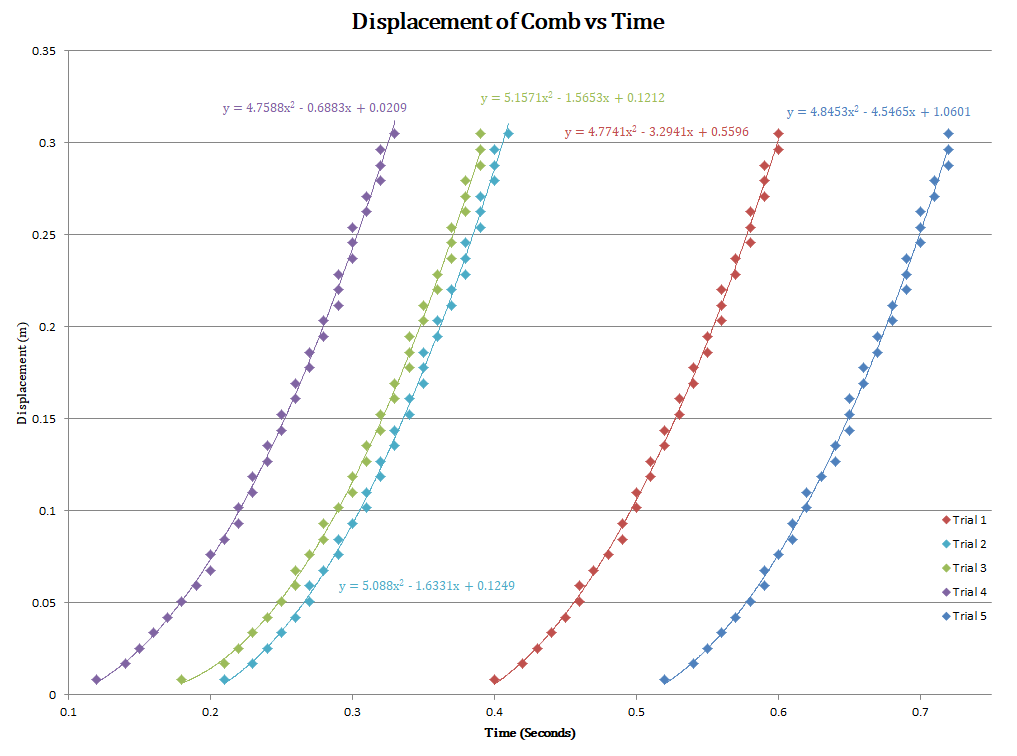
\includegraphics[width=5.0in]{CombGraph.png}
    \caption{Scatterplot of displacement of the comb graphed against elapsed time, over 4 seperate trials. Fit lines are quadratic and provided by Microsoft Excel.}
\end{figure}

Using the general case formula for displacement given a constant acceleration, we can find the acceleration due to gravity on the comb. The equation is provided below:

\begin{align}
     \Delta x = v_ot+\frac{1}{2}at^2
\end{align}

Using that equation, we can find the accelerations for the four different trials by multiplying the coefficient of the $x^2$ term by a factor of two, giving the following accelerations due to gravity: 9.55 m/s$^2$, 10.18 m/s$^2$, 10.31 m/s$^2$, 9.52 m/s$^2$, and 9.69 m/s$^2$.

However, these values are incomplete as they lack uncertainty of \textit{g}. Using Excel's regression tool, we solve for the uncertainty in the quadratic coefficient. For the previous values, the statistical uncertainties of $g$ are respectively $\pm$ 0.28 m/s$^2$, $\pm$ 0.27 m/s$^2$, $\pm$ 0.27 m/s$^2$, $\pm$ 0.31 m/s$^2$, and $\pm$ 0.29 m/s$^2$. 

This analysis of $\delta g$, however, is incomplete as it does not account for systematic uncertainties. To account for systematic uncertainties, we account for the fact that $\lambda$ also has an uncertainty of $\pm$ 0.5 mm. Using the method similar to what was used to account for systematic uncertainties in the ball drop experiment, we perform linear regressions for the data set using the maximum and minimum values for $\lambda$, find the difference between the maximum and minimum $g$ values, and divide it by two to solve for the systematic uncertainty.

\begin{align}
    \delta g = \frac{g\textsubscript{max} - g\textsubscript{min}}{2}
\end{align}

The value of systematic uncertainty for all four trials is  $\pm$ 0.006 m/s$^2$. From this we can safely ignore the systematic uncertainty of $g$ when calculating $\delta g$ as the order of magnitude of the systematic uncertainty is far less than that of the statistical uncertainty. Consequently, when taking into account significant figures, the systematic uncertainty values would be truncated when put into comparison with the statistical uncertainty values. This leads us to final measured accelerations, displayed in the table below:

\begin{table}[!htbp]
\renewcommand{\arraystretch}{1.3}
\centering
\begin{tabular}{c|c}
    \hline
    \hline
    Trial Number & \textit{g} with Uncertainty (m/s$^2$)\\
    \hline
    \hline

    1    &  9.55 $\pm$ 0.28 \\
    \hline

    2    &  10.18 $\pm$ 0.27 \\
    \hline

    3   &   10.31 $\pm$ 0.27\\
    \hline

    4   &  9.52 $\pm$ 0.31\\
    \hline

    5  &  9.69 $\pm$ 0.29\\
    \hline
\end{tabular}
\caption{Measured accelerations due to gravity and their respective optained via usage of the regression tool in Microsoft Excel. Systematic uncertainty was not included in total uncertainty as it is more than ten times less in value than the statistical uncertainty. }
\end{table}

\pagebreak

\section{Conclusion}
While the values obtained from the various tests for $g$ were not exactly 9.8 m/s$^2$, the widely accepted constant for gravitational acceleration on Earth, the best value we obtained for the ball drop was only 0.05 m/s$^2$ off and the best value for the photogate comb drop was 0.11 m/s$^2$ off (0.0545 m/s$^2$ and 0.1055 m/s$^2$, respectively, in comparison to the acceleration due to gravity at Knudsen 1-238: (9.7955 $\pm$ 0.0003) m/s$^2$).

\begin{table}[!htbp]
\renewcommand{\arraystretch}{1.3}
\centering
\begin{tabular}{c|c}
    \hline
    \hline
    Ball Drop \textit{g} (m/s$^2$) & Photogate Comb \textit{g} (m/s$^2$)\\
    \hline
    \hline

    9.48 $\pm$ 0.20 &  9.52 $\pm$ 0.31\\
    \hline

    9.73 $\pm$ 0.18 & 9.55 $\pm$ 0.28 \\
    \hline

    9.85 $\pm$ 0.16 &  9.69 $\pm$ 0.29 \\
    \hline

    10.12 $\pm$ 0.37 & 10.18 $\pm$ 0.27 \\ 
    \hline

    10.38 $\pm$ 0.22 & 10.31 $\pm$ 0.27 \\
    \hline
\end{tabular}
\caption{Calculated values for \textit{g} for both the ball drop method and the photogate comb method, organized from lowest to highest. Row 3 represents the closest values to the "true" acceleration due to gravity for both methods. The \textit{D} values for the ball drop column are in the following order: 563 $\pm$ 1 mm, 448 $\pm$ 1 mm, 653 $\pm$ 1 mm, 243 $\pm$ 1 mm, and 381 $\pm$ 1 mm. }
\end{table}

While the ball drop method ended with the closest value to the true acceleration due to gravity, it at the same time suffered from higher systematic uncertainty and had some additional statistical uncertainty, while the source of uncertainty for the comb method was statistical uncertainty, as the systematic uncertainty was comparably negligible. If we were to assume that for the ball drop method that the uncertainty is accurate to only a single value beyond the decimal point, the statistical uncertainty could be theoretically ignored.

Consequently, if the test were performed with a longer comb with more photogates, thereby increasing the number of data points per trial and thereby reducing statistical uncertainty, the photogate comb method would provide a more precise and accurate result. For the ball drop method however, there is a trend in that the greater $D$ is, the lower the systematic uncertainty is. However, given the limitation of the fact that a meterstick was used to measure $D$, the uncertainty of $D$ would rise significantly for values greater than 1 meter.

Therefore, in the case of this particular setup of Experiment 2, the ball drop method is more accurate and precise for larger values of $D$. However, given a longer photogate comb with more slots, the photogate method may very well be far more precise, as the primary source of uncertainty for the photogate comb method is statistical uncertainty, which decreases with more data values. 

\pagebreak

\section{Extra Credit}
One of the primary drawbacks of the photogate comb method is keeping the comb vertical as it drops in order to obtain an accurate method of $g$. In an attempt to combat the potential swinging of the comb, a paper strip was looped through the top photogate, allowing the comb to stabalize, before one end of the strip was released, allowing the comb to drop. Applying the same regression techniques as used for the other photogate comb drops, and comparing the values with the "best" photogate drop trial, we are presented with the following table:

\begin{table}[!htbp]
\renewcommand{\arraystretch}{1.3}
\centering
\scalebox{0.8}
{
\begin{tabular}{c|c|c}
    \hline
    \hline
    Calculated \textit{g} (m/s$^2$) & Statistical Uncertainty of \textit{g} (m/s$^2$) & Systematic Uncertainty of \textit{g} (m/s$^2$)\\
    \hline
    \hline

    9.96 &  $\pm$ 0.26 &  0.006 m/s$^2$\\
    \hline

    9.69 & $\pm$ 0.29 &  0.006 m/s$^2$ \\
    \hline
\end{tabular}
}
\caption{Comparison of the paper strip photogate comb drop (Row 1) with the normal photogate comb drop (Row 2). The trial used for the normal photogate drop was Trial 5 (see Figure 4). Trial 5 was selected as its calculated $g$ is closest to the true acceleration due to gravity.}
\end{table}

From this data we can see that the resultant values for the photogate comb drop remain nonetheless similar regardless of which method was used to perform the test, and that the statistical uncertainty remains dominant. We can therefore still conclude that the primary drawback of the photogate comb drop remains the shortness of the comb which limits the data points that can be obtained per drop.

Furthermore, assuming uniform density, a longer photogate comb would move the center of gravity farther from the potential pivot point of the comb, being the end of the comb being held, and increase its mass, thereby increasing the force of gravity on the comb and the length of the lever arm. Consequently it would allow gravity to apply more torque on the comb if it were not already vertical, further stabilizing the comb and aiding in keeping it vertical.

Therefore, the limitations of the photogate comb drop arise from the setup itself, rather than the execution of the drop.

\pagebreak

\begin{thebibliography}{1}
\bibitem{a}
Campbell, W. C. \textit{et al}. Physics 4AL: Mechanics Lab Manual (ver. April 3, 2017).
(Univ. California Los Angeles, Los Angeles, California).
\end{thebibliography}

\end{document}
T